\documentclass[a4paper,11pt,oneside,openany]{book}

\usepackage[left=30mm,right=30mm,top=25mm,bottom=25mm]{geometry}
\usepackage{cscover}
\usepackage[dvipdfmx]{graphicx}
\usepackage[nobreak]{cite}
\usepackage[a4paper,dvipdfmx,pdfdisplaydoctitle=true,%
    bookmarks=true,bookmarksnumbered=true,bookmarkstype=toc,bookmarksopen=true,%
    pdftitle={A Study on Thesis Formats},%
    pdfauthor={Taro Tokodai}%
    ]{hyperref}

\renewcommand{\bibname}{References}
\pagestyle{plain}
\thesistype{Master's Thesis}
%\thesistype{Doctoral Dissertation}
\title{High-Frequency Trading trader's order frequency analysis using Multi-Hawkes Process}
\author{Hiroki Watari}
\studentid{20M30462}
\affiliation{%
  %Graduate Major in Computer Science\\
  Graduate Major in Artificial Intelligence\\
  School of Computing\\
  Tokyo Institute of Technology}
\date{January, 2021}

\supervisorname{Supervisor:}
\supervisor{Misako Takayasu}
%\dsupervisorname{Deputy Supervisor:}
%\dsupervisor{Jiro Kogaku}

\begin{document}
\frontmatter
\maketitle
\chapter{Abstract}
情報技術の発展を背景とした金融市場の高頻度化が進み、それに伴い高頻度金融データと呼ばれる取引単位の詳細なデータが蓄積され利用可能になりました。これを背景として、金融市場に参加するトレーダーがどのような戦略に従い取引を行っているのか。そして彼らの取引戦略が市場価格の形成にどのような役割を果たしているのかということも詳細に研究が行われるようになってきています。\\
トレーダーの取引戦略と市場価格形成を関係付けた経済物理学の代表的な事例の1つとして、データドリブンに個々のトレーダーの取引行動をモデル化し、板の発生、そして市場価格形成の関係までを理論的に明らかにした事例が挙げられます。 金融市場の高頻度化、及び詳細なトレーダーの取引行動の解析が近年可能になったことも背景として存在しており、高頻度金融データの解析は今後も研究の需要と可能性が高い分野だと考えられます。\\
そこで本研究では超高速取引トレーダー(以下、HFT)の取引行為がどのように行われているのかを理解することを目的として、ドル円の外国為替市場に参加している個々のHFTトレーダーの注文頻度の解析を行います。具体的には、HFTトレーダーの買い注文と売り注文がどのようなタイミングで注文されている傾向にあるのかを、多次元hawkes過程を用いて解析しました。\\
その結果、多くのHFTトレーダーの買い注文は市場全体の買い注文発生と売り注文キャンセル時、HFTトレーダーの買い注文は市場全体の売り注文発生と買い注文キャンセル時に発生する傾向にある示唆を得たことを報告します。

hhhhh
hsss
cndlcn
sdlnk

\tableofcontents
%%\listoffigures
%%\listoftables

%%%%%%%%%%%%%%%%%%%%%%%%%%%%%%%%%%%%%%%%%%%%%%%%%%
\chapter{1 Introduction}
近年,情報通信技術の発達や情報処理機器の高性能化に伴い,世界中の金融市場において取引システムの高速化や,取引データの時間解像度の向上が図られている.

HFTトレーダーに対して多次元Hawkes過程でモデル化した事例は筆者が知る存在しない。本研究の実証結果はその意味においては最初の研究と位置づけられる.



本研究の構成は以下の通りである.セクション2では、本研究で使用するデータ及びHFTトレーダーの説明を行う.セクション3では,多次元Hakweks過程の導入及び最適化手法について記述する.セクション4では,実証分析の結果とその解釈について議論する.セクション5ではモデルの妥当性について言及最後に,セクション5は本論文の結言である.
I introduce a sample of how to write a thesis\cite{1}.


\section*{1.1 Sample}


\begin{equation}
  r^2 = \sum_{k=1}^{n} x_k^2 \label{eq:hs}
\end{equation}


According to Table~\ref{tab:sample}, it has four elements $(a, b, c, d)$.
\begin{table}[htb]
  \centering
  \caption{Elements}\label{tab:sample}
  \begin{tabular}{|c|r|}
    \hline
    $a$ & $b$ \\ \hline
    $c$ & $d$ \\ \hline
  \end{tabular}
\end{table}

%%%%%%%%%%%%%%%%%%%%%%%%%%%%%%%%%%%%%%%%%%%%%%%%%%

\chapter{2 Data Description}
本研究では,EBSが提供するUSD/JPY市場の高頻度注文送信および取引データを使用します。 EBSのUSD/JPY市場の高頻度注文と取引データを使用します。このデータは2016年6月5日から6月10日までの1週間を対象としており,その間に約 300万件の注文が提出されました。このデータセットでは、各レコードには価格だけでなく、数量。とタイムスタンプ(ミリ秒単位)だけでなく、匿名化されたトレーダーと銀行のIDも含まれています。これらのIDは これらのIDは匿名化されていますが、この期間中は固定されているため、特定のトレーダーや銀行による取引の完全な履歴を追跡することができます。特定のトレーダーや銀行の1週間の取引履歴を追跡することができます。トレーダーが指定できる最小価格単位は0.005円、最小送信量は100万ドルです。ここでは、価格単位を0.001円のtpipとします(すなわち、トレーダーが指定できる最小価格単位は5tpip)。価格単位は0.001円のtpip(トレーダーが指定できる最小価格単位は5tpip)、数量は100万ドルの倍数とします。合計で、335の銀行が この週に行われた取引の総額は約680億ドルでした。
\begin{figure}[htb]
  \centering
  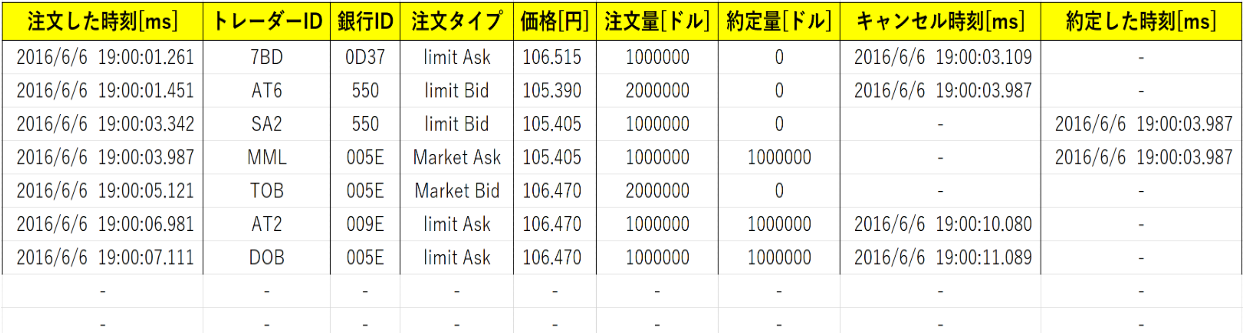
\includegraphics[scale=0.7]{./figures/table_data.png}
  \caption{テーブルデータの例}\label{fig:hs}
\end{figure}
\section*{2.1 Short review our analysis}
本研究ではEBS社提供のspot取引のデータを使用する。


\section*{2.2 High-Frequency Trader}
\begin{figure}[htb]
  \centering
  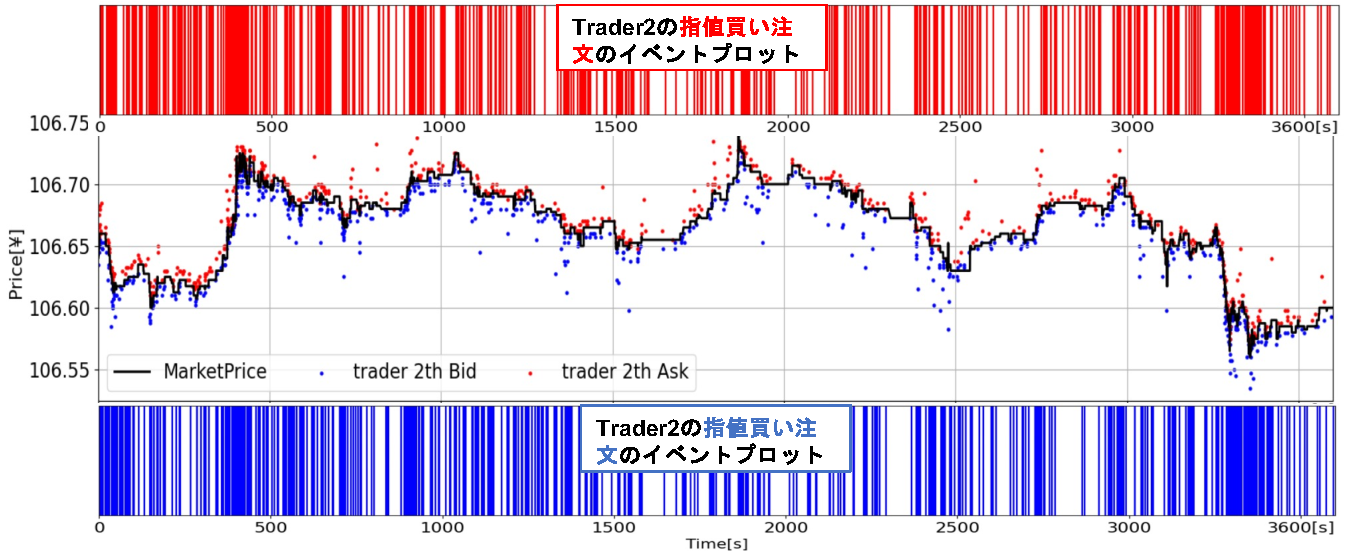
\includegraphics[scale=0.7]{./figures/order_sample.pdf}
  \caption{テーブルデータの例}\label{fig:hs}
\end{figure}


%%%%%%%%%%%%%%%%%%%%%%%%%%%%%%%%%%%%%%%%%%%%%%%%%%

\chapter{3 Method}
\section*{3.1 Short review our analysis}

%%%%%%%%%%%%%%%%%%%%%%%%%%%%%%%%%%%%%%%%%%%%%%%%%%

\chapter{4 Result}
\section*{3.1 Short review our analysis}

%%%%%%%%%%%%%%%%%%%%%%%%%%%%%%%%%%%%%%%%%%%%%%%%%%

\appendix
\chapter{Proof of Theorem 1}
Appendices can be added.

%%%%%%%%%%%%%%%%%%%%%%%%%%%%%%%%%%%%%%%%%%%%%%%%%%

\backmatter
\chapter{Acknowledgment}
Thank you.

%%%%%%%%%%%%%%%%%%%%%%%%%%%%%%%%%%%%%%%%%%%%%%%%%%

\bibliographystyle{plain}
\bibliography{references-e}
%\begin{thebibliography}{99}
%  \bibitem{tokodai-xyz2015} Taro Tokodai. How to write a good thesis. \textit{Journal of XYZ}, 3(4):15--34, 2015.
%\end{thebibliography}

\end{document}
